% Charlotte Geiger - Manuel Lippert - Leonard Schatt
% Physikalisches Praktikum

% Teilauswertung 1

\section{Eingangskennlinie des Transistors}
Bei der Auswertung der Eingangskennlinie des Transistors interessiert uns der Graph $I_B(U_{BE})$, welcher die Eingangskennlinie beschreiben soll. Bei der Messaufgabe 1 haben wir die Kennlinie folgender Schaltung gemessen:
\begin{center}
    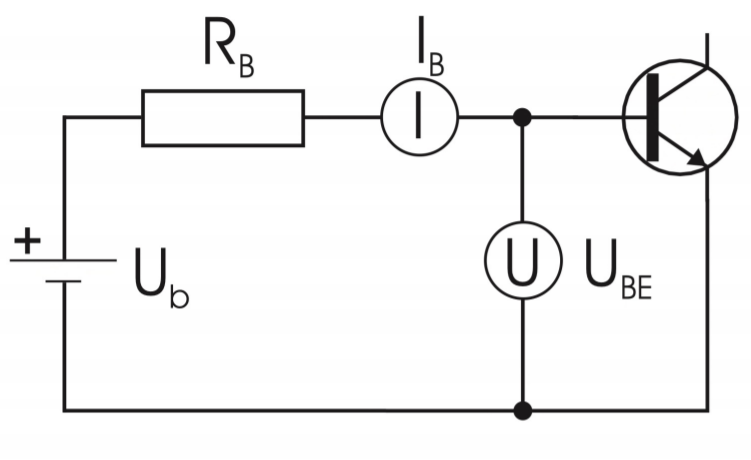
\includegraphics[scale=0.5]{6_1-Schaltung.PNG}
    %\captionof{figure}{Schaltung für Eingangs}
\end{center}
Zu messen sind hierbei $I_B$ und $U_{BE}$ mit je einem DMM im Bereich $I_B=0,01 bis 4 \text{mA}$. Für die Berechnungen sind zuerst die Fehler wichtig. Die Ablesefehler sind jeweils 0,5 Digits. Somit folgt die Rechnung:
\begin{equation}
    s_{I_B}=\sqrt{s_r^2+0,005^2}
\end{equation}
\newpage
Somit ergeben sich folgende Tabellen und Graphen:
\begin{center}
    \captionof{table}{Messreihe mit Fehler}
    \begin{tabular}{l|cccc}
        {} &     $I_B/\text{mA}$ &   $s_{I_B}/\text{mA}$ &     $U_{BE}/\text{V}$ &   $s_{U_{BE}}/\text{V}$ \\
        \hline
        1  &  0.01 &     0.03 &  0.559 &     0.007 \\
        2  &  0.02 &     0.03 &  0.578 &     0.008 \\
        3  &  0.03 &     0.03 &  0.587 &     0.008 \\
        4  &  0.04 &     0.03 &  0.593 &     0.008 \\
        5  &  0.05 &     0.03 &  0.600 &     0.008 \\
        6  &  0.08 &     0.03 &  0.614 &     0.008 \\
        7  &  0.10 &     0.03 &  0.620 &     0.008 \\
        8  &  0.15 &     0.03 &  0.635 &     0.008 \\
        9  &  0.20 &     0.03 &  0.644 &     0.008 \\
        10 &  0.25 &     0.03 &  0.651 &     0.008 \\
        11 &  0.30 &     0.03 &  0.657 &     0.008 \\
        12 &  0.35 &     0.03 &  0.663 &     0.008 \\
        13 &  0.40 &     0.04 &  0.667 &     0.008 \\
        14 &  0.45 &     0.04 &  0.671 &     0.008 \\
        15 &  0.50 &     0.04 &  0.675 &     0.008 \\
        16 &  0.55 &     0.04 &  0.678 &     0.008 \\
        17 &  0.60 &     0.04 &  0.682 &     0.008 \\
        18 &  0.65 &     0.04 &  0.684 &     0.008 \\
        19 &  0.70 &     0.04 &  0.687 &     0.008 \\
        20 &  0.75 &     0.04 &  0.690 &     0.008 \\
        21 &  0.80 &     0.04 &  0.692 &     0.008 \\
        22 &  0.85 &     0.04 &  0.694 &     0.008 \\
        23 &  0.90 &     0.04 &  0.696 &     0.008 \\
        24 &  0.95 &     0.04 &  0.698 &     0.008 \\
        25 &  1.00 &     0.04 &  0.700 &     0.008 \\
        26 &  1.10 &     0.04 &  0.703 &     0.008 \\
        27 &  1.20 &     0.04 &  0.706 &     0.008 \\
        28 &  1.30 &     0.05 &  0.709 &     0.008 \\
        29 &  1.40 &     0.05 &  0.711 &     0.008 \\
        30 &  1.50 &     0.05 &  0.714 &     0.008 \\
        31 &  1.60 &     0.05 &  0.716 &     0.008 \\
        32 &  1.70 &     0.05 &  0.718 &     0.008 \\
        33 &  1.80 &     0.05 &  0.720 &     0.008 \\
        34 &  1.90 &     0.05 &  0.722 &     0.008 \\
        35 &  2.00 &     0.05 &  0.724 &     0.008 \\
        36 &  2.50 &     0.06 &  0.732 &     0.008 \\
        37 &  3.00 &     0.07 &  0.738 &     0.009 \\
        38 &  3.50 &     0.07 &  0.744 &     0.009 \\
        39 &  4.00 &     0.08 &  0.749 &     0.009 \\
    \end{tabular}
\end{center}
\begin{center}
    \captionof{figure}{$I_B-U_{BE}$ Diagramm - Eingangskennlinie Transistor}
    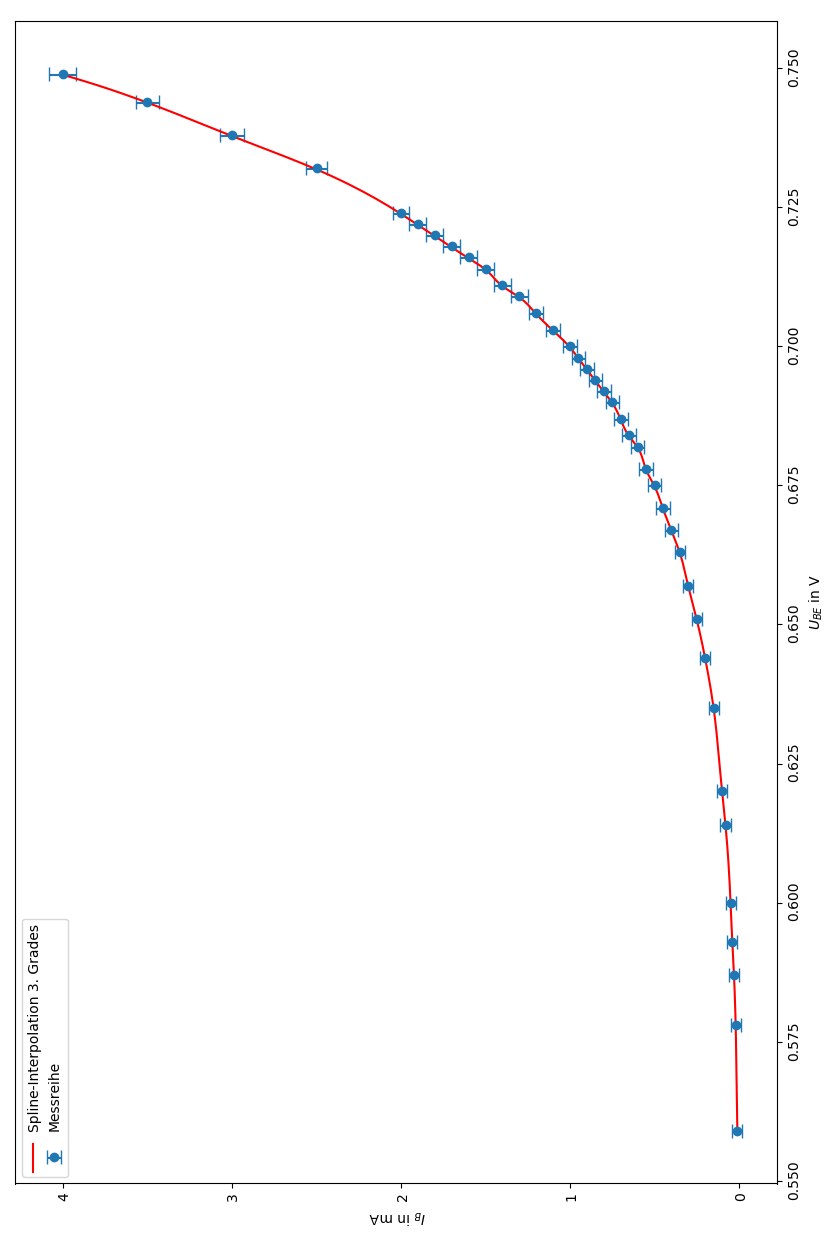
\includegraphics[scale=0.6]{6_1-Kennlinie.png}
\end{center}
Da die Funktion nach ihrer Schleusenspannung einen extremen Anstieg aufweist, sieht man sehr gut, dass folgende analytische Funktion die Form der gemessenen Graphen gut beschreibt: 
\begin{equation}
    exp[\alpha(x-\beta)^2]-1
\end{equation}
Nun berechnen und bestimmen wir den Verlauf der differenziellen Eingangswiderst\"ande $r_{BE}$
Der Differentielle Widerstand beschreibt ein Maß für die Stromänderung, wenn Spannung am Bauteil geringfügig geändert wird. Dieser kann durch die Ableitung der Kennlinie berechnet werden, oder man kann diesen funktionellen Zusammenhang auch aus den Differenzen benachbarter Messwertpaare $U_{BE}^i, I_B^i$ und $U_{BE}^{i+1},  I_B^{i+1}$ beschreiben.
\begin{align}
    r_{BE}=\frac{dU_{BE}}{dI_B}\approx\frac{\Delta U_{BE}}{\Delta I_B}=\frac{U_{BE}^{i+1}-U_{BE}^i}{I_B^{i+1}-I_B^i}
\end{align}
Der Fehler wird mit dem Fehlerfortpflanzungsgesetz ermittelt und ist gegeben als
\begin{gather}
    s_{r_{BE}}=\sqrt{\left(\frac{1}{\Delta I_B}s_{\Delta U_{BE}}\right)^2+\left(\frac{\Delta U_{BE}}{\Delta I_B^2}s_{\Delta I_B}\right)^2}\\[0.3cm]
    \text{mit}\tab s_{\Delta I_B}=\sqrt{s_{I^{i+1}_B}^2+s_{I^{i}_B}^2}\tab s_{\Delta U_{BE}}=\sqrt{s_{U^{i+1}_{BE}}^2+s_{U^{i}_{BE}}^2}
\end{gather}
Die Erwartung hierbei ist, je größer der Strom ist, desto geringer der Widerstand, da der Coulomb-Wall für kleinere Ströme nicht gut genug abgebaut wird und daher die Diffusion der Ladungsträger nicht überbrückt werden und somit der Stromfluss nicht so gut ist. \\
\\ Bei der Berechnung ist auffällig, dass der Fehler $s_{r_{BR}}$ sehr groß ist für niedrige Basisstromänderungen $\Delta I_B$ und kontinuierlich abnimmt, wenn sie $\Delta I_B$ zunimmt. Das ist offensichtlich da $\Delta I_B$ in 4. Potenz im Fehler $s_{r_{BR}}$ eingeht. Zur Übersicht wurden darauf verzichtet die ersten vier berechneten werte von $s_{r_{BR}}$ in den Plot einzufügen. Weiterhin wird $r_{BE}$ gegen $I_B$ aufgetragen, da aber $r_{BE}$ durch die Berechnung nur 38 Werte besitzt, muss $I_B$ mit 39 Messwerte ein Datenpunkt entfernt werden. Durch die Konstruktion der Werte für $r_{BE}$ wird hier die $I^i_B$ Stützstellen verwendet.
\newpage
\begin{center}
    \captionof{table}{Differentielle Widerstand}
    \begin{tabular}{l|cccc|ccc}
        {}  &  $\Delta I_{B}/\text{mA}$ &   $s_{\Delta I_{B}}/\text{mA}$ & $\Delta U_{BE}/\text{V}$ &   $s_{\Delta U_{BE}}/\text{V}$ &     $r_{BE}/\text{k} \Omega$ &   $s_{r_{BE}}/\text{k} \Omega$ & $I_B/\text{mA}$ \\ 
        \hline    
        1  &     0.01 &         0.04 &     0.019 &         0.011 &  1.900 &      8.13 &  0.01 \\      
        2  &     0.01 &         0.04 &     0.009 &         0.011 &  0.900 &      3.98 &  0.02 \\      
        3  &     0.01 &         0.04 &     0.006 &         0.011 &  0.600 &      2.79 &  0.03 \\      
        4  &     0.01 &         0.04 &     0.007 &         0.011 &  0.700 &      3.18 &  0.04 \\      
        5  &     0.03 &         0.04 &     0.014 &         0.011 &  0.467 &      0.76 &  0.05 \\      
        6  &     0.02 &         0.04 &     0.006 &         0.011 &  0.300 &      0.85 &  0.08 \\      
        7  &     0.05 &         0.04 &     0.015 &         0.011 &  0.300 &      0.34 &  0.10 \\      
        8  &     0.05 &         0.04 &     0.009 &         0.011 &  0.180 &      0.27 &  0.15 \\      
        9  &     0.05 &         0.04 &     0.007 &         0.011 &  0.140 &      0.26 &  0.20 \\      
        10 &     0.05 &         0.04 &     0.006 &         0.011 &  0.120 &      0.25 &  0.25 \\      
        11 &     0.05 &         0.04 &     0.006 &         0.011 &  0.120 &      0.25 &  0.30 \\      
        12 &     0.05 &         0.05 &     0.004 &         0.011 &  0.080 &      0.24 &  0.35 \\      
        13 &     0.05 &         0.06 &     0.004 &         0.011 &  0.080 &      0.24 &  0.40 \\      
        14 &     0.05 &         0.06 &     0.004 &         0.011 &  0.080 &      0.24 &  0.45 \\      
        15 &     0.05 &         0.06 &     0.003 &         0.011 &  0.060 &      0.24 &  0.50 \\      
        16 &     0.05 &         0.06 &     0.004 &         0.011 &  0.080 &      0.24 &  0.55 \\      
        17 &     0.05 &         0.06 &     0.002 &         0.011 &  0.040 &      0.23 &  0.60 \\      
        18 &     0.05 &         0.06 &     0.003 &         0.011 &  0.060 &      0.24 &  0.65 \\      
        19 &     0.05 &         0.06 &     0.003 &         0.011 &  0.060 &      0.24 &  0.70 \\      
        20 &     0.05 &         0.06 &     0.002 &         0.011 &  0.040 &      0.23 &  0.75 \\      
        21 &     0.05 &         0.06 &     0.002 &         0.011 &  0.040 &      0.23 &  0.80 \\      
        22 &     0.05 &         0.06 &     0.002 &         0.011 &  0.040 &      0.23 &  0.85 \\      
        23 &     0.05 &         0.06 &     0.002 &         0.011 &  0.040 &      0.23 &  0.90 \\      
        24 &     0.05 &         0.06 &     0.002 &         0.011 &  0.040 &      0.23 &  0.95 \\      
        25 &     0.10 &         0.06 &     0.003 &         0.011 &  0.030 &      0.11 &  1.00 \\      
        26 &     0.10 &         0.06 &     0.003 &         0.011 &  0.030 &      0.11 &  1.10 \\      
        27 &     0.10 &         0.06 &     0.003 &         0.011 &  0.030 &      0.11 &  1.20 \\      
        28 &     0.10 &         0.07 &     0.002 &         0.011 &  0.020 &      0.11 &  1.30 \\      
        29 &     0.10 &         0.07 &     0.003 &         0.011 &  0.030 &      0.12 &  1.40 \\      
        30 &     0.10 &         0.07 &     0.002 &         0.011 &  0.020 &      0.11 &  1.50 \\      
        31 &     0.10 &         0.07 &     0.002 &         0.011 &  0.020 &      0.11 &  1.60 \\      
        32 &     0.10 &         0.07 &     0.002 &         0.011 &  0.020 &      0.11 &  1.70 \\      
        33 &     0.10 &         0.07 &     0.002 &         0.011 &  0.020 &      0.11 &  1.80 \\      
        34 &     0.10 &         0.07 &     0.002 &         0.011 &  0.020 &      0.11 &  1.90 \\      
        35 &     0.50 &         0.08 &     0.008 &         0.011 &  0.016 &      0.02 &  2.00 \\      
        36 &     0.50 &         0.09 &     0.006 &         0.012 &  0.012 &      0.02 &  2.50 \\      
        37 &     0.50 &         0.10 &     0.006 &         0.013 &  0.012 &      0.03 &  3.00 \\      
        38 &     0.50 &         0.11 &     0.005 &         0.013 &  0.010 &      0.03 &  3.50 \\
    \end{tabular}
\end{center}
\newpage
\begin{center}
    \captionof{figure}{$I_B-r_{BE}$ Diagramm - Differentielle Widerstand}
    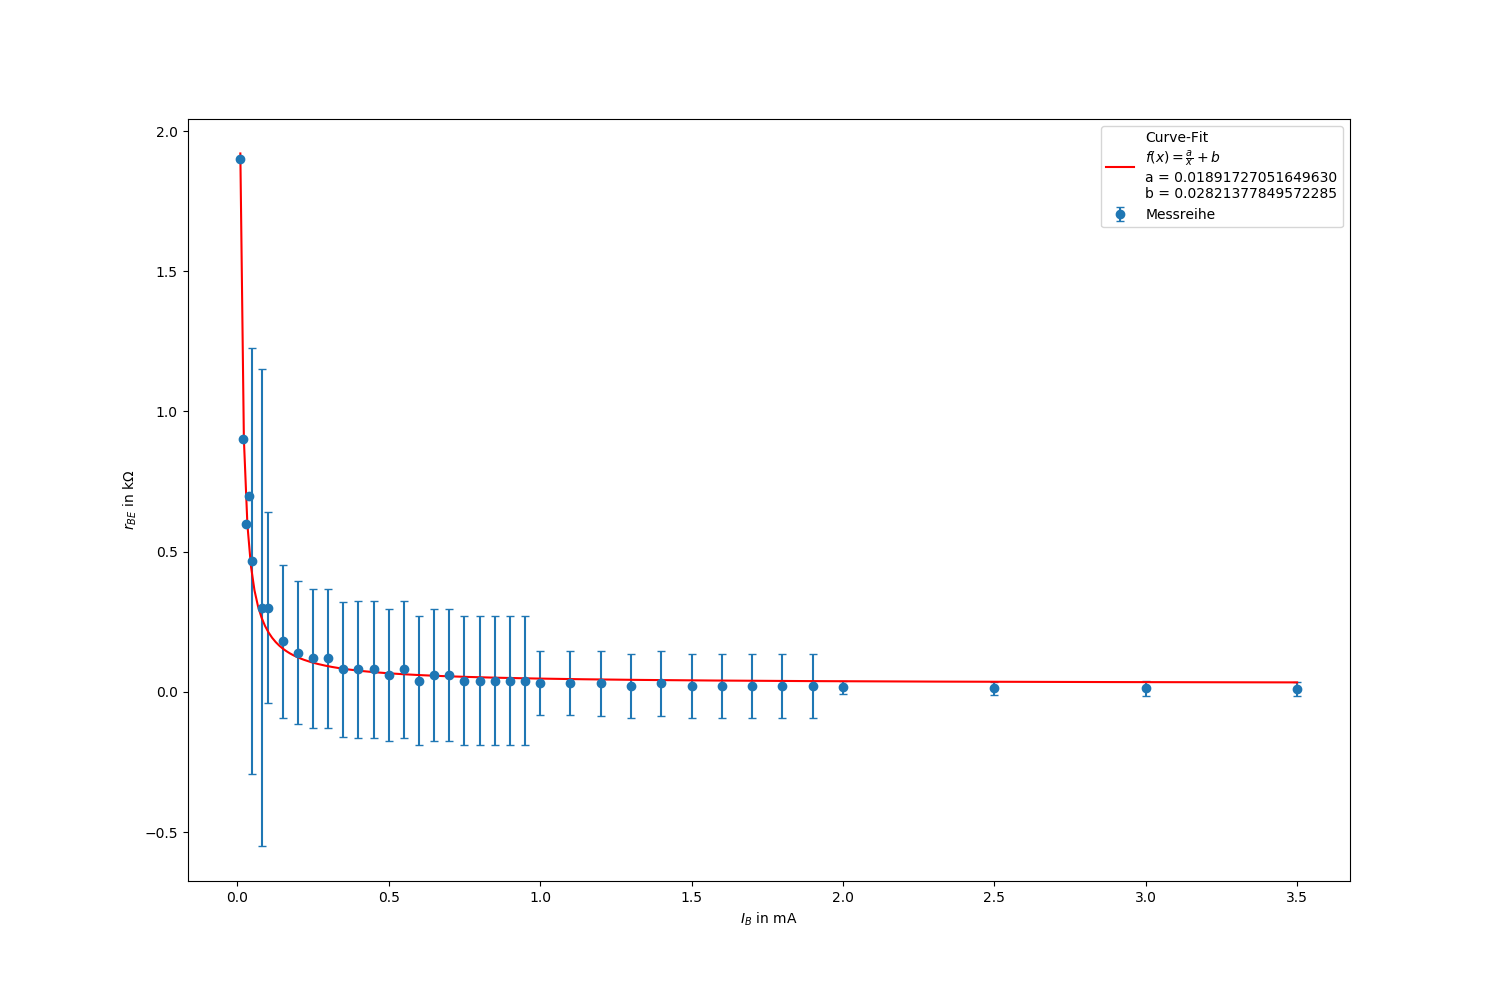
\includegraphics[scale=0.6]{6_1-Diff_Widerstand.png}
\end{center}
\newpage